\documentclass{article}

\usepackage[includehead,top=0.9in,bottom=0.9in,left=1in,right=1in]{geometry}
% Macro for homework

% Preamble and packages 
\usepackage{lipsum}
\usepackage{amsmath,amsfonts,amsthm}
\usepackage{graphicx}

% General
\def\R{{\mathbb{R}}}

% Probability
\def\P{{\mathbb{P}}}
\def\E{{\mathbb{E}}}



\title{\textbf{Homework Assignment Title}}
\author{Chuyang Ke}
\date{\today}

\usepackage[parfill]{parskip}   % no paragraph indent, add paragraph spacing
\begin{document}

\maketitle

% Preamble ends here

\section{Texts}

Here are some texts. Here are some texts. Here are some texts.

Here are some texts. Here are some texts. Here are some texts.

Here are some texts. Here are some texts. Here are some texts.

\lipsum[1]


\section{Equations}

We can use the inline mode 
$1 + 1 = 2$, 
or display mode
\[
1 + 1 = 2 \,,    
\]
for the same equation.

We can use $\P(x)$ for probability, $\E(x)$ for expectation. $\R$ denotes the set of real numbers.


\section{Lists}
We can use numbered lists:
\begin{enumerate}
    \item First, \dots
    \item Second, \dots
\end{enumerate}
Or bullet points:
\begin{itemize}
    \item First, \dots
    \item Second, \dots
\end{itemize}


\section{Figures}
Figure \ref{fig:example} is an example image.
\begin{figure}[h]
    \centering
    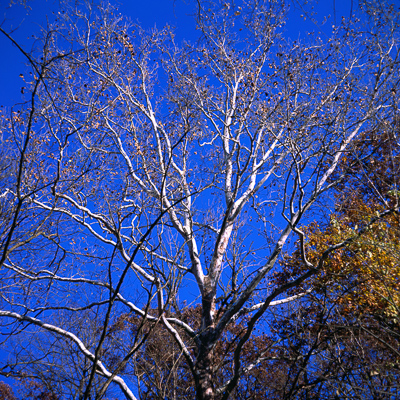
\includegraphics[width=0.25\linewidth]{figs/example.jpg}
    \caption{Caption}
    \label{fig:example}
\end{figure}


% \section{Algorithms}

% Document ends here
\end{document}


